\subsection{\label{sec:calib.trig.eff}Trigger Efficiency}

In the first few weeks of \desg{g12}, during ``commissioning,'' an attempt to determine the efficiency of the two-track trigger (bit 8 in Tables.~\ref{tab:data.trig.conf.1} and \ref{tab:data.trig.conf.2}) was made. The rate of this main production trigger rose quadratically with the beam current while the physical event rate increased linearly. The number of accidentals, which must be cut from any analysis, increased with increasing current and at a certain point, the majority of the events taken were accidentals. The trigger rate as a function of the beam current is shown in Fig.~\ref{fig:data.trig.eff}. An estimate of the linear part of the trigger rate shows that approximately 60\% of the events recorded during the \desg{g12} experiment (which ran at 60--65~nA beam current) were accidentals.

\begin{figure}\begin{center}
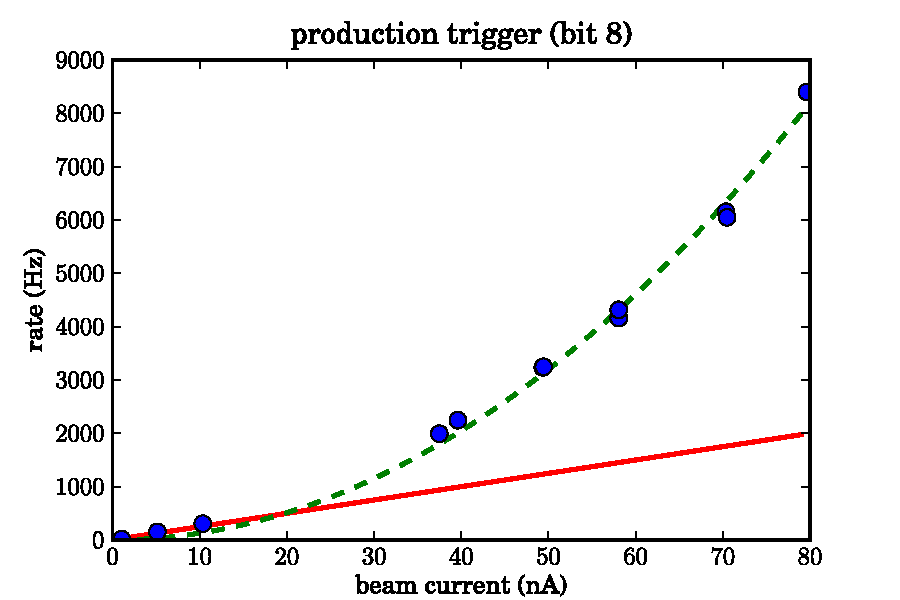
\includegraphics[width=0.6\columnwidth]{figures/calib/trig/trigger_study.eps}
\caption[Trigger Rate vs. Beam Current]{\label{fig:data.trig.eff}The production trigger rate (bit 8 in Tables~\ref{tab:data.trig.conf.1} and \ref{tab:data.trig.conf.2}) was measured for various beam currents shown by the blue dots. The rates below 10~nA are roughly linear and are extrapolated via the red solid line to show an estimate of the physical event rate. The actual trigger rate is fitted with a quadratic shown by the green dashed line. By this estimate, the accidental rate is shown to equal the physical event rate at approximately 40~nA. The \desg{g12} experiment was done at 60--65~nA.}
\end{center}\end{figure}

\FloatBarrier
